\documentclass[border=8pt]{standalone}
\usepackage{amsmath}
\usepackage{tikz}
\usetikzlibrary{arrows.meta,calc}
\begin{document}
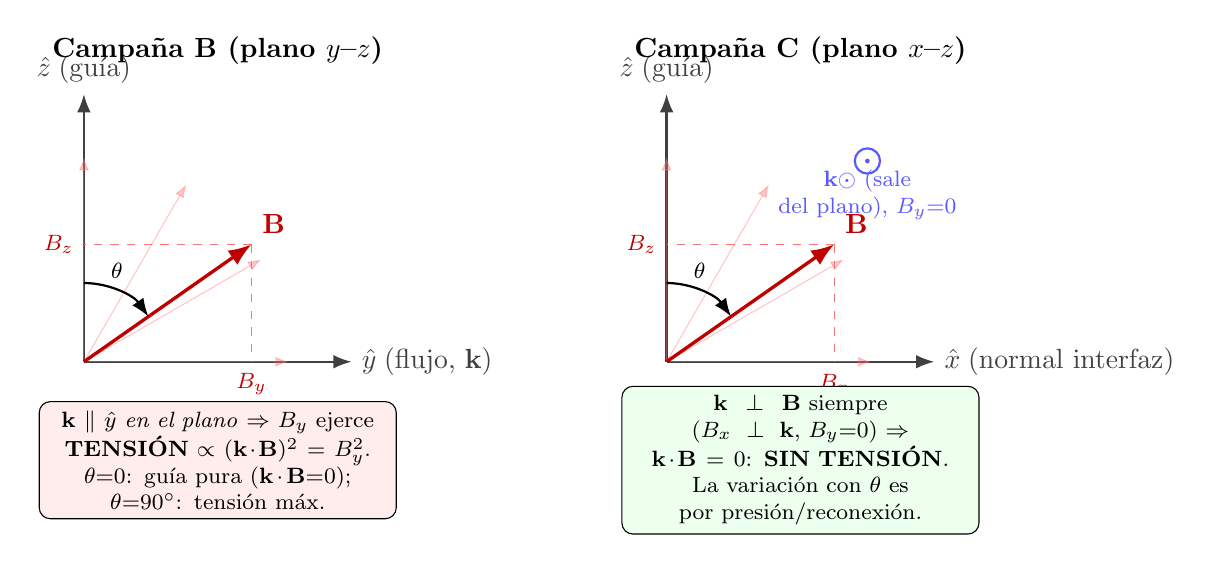
\begin{tikzpicture}[>=Latex,scale=1.0,
  ax/.style={->,thick,black!75},
  Bvec/.style={->,very thick,red!75!black},
  Bfaint/.style={->,red!55,opacity=0.40},
  comp/.style={red!55,dashed}]

\def\R{2.6}      % radio (|B|)
\def\tb{55}      % angulo representativo

% =================== PANEL B (plano y-z) ===================
\begin{scope}
  \coordinate (O) at (0,0);
  % ejes del plano de rotacion
  \draw[ax] (O) -- (3.4,0) node[right] {$\hat y$\;(flujo, $\mathbf k$)};
  \draw[ax] (O) -- (0,3.4) node[above] {$\hat z$\;(guía)};
  % familia de B (theta desde z hacia y)
  \foreach \t in {0,30,60,90}{
    \draw[Bfaint] (O) -- ({\R*sin(\t)},{\R*cos(\t)});
  }
  % B representativo
  \coordinate (B) at ({\R*sin(\tb)},{\R*cos(\tb)});
  \draw[Bvec] (O) -- (B) node[above right] {$\mathbf B$};
  % componentes By (horizontal), Bz (vertical)
  \draw[comp] (B) -- ({\R*sin(\tb)},0);
  \draw[comp] (B) -- (0,{\R*cos(\tb)});
  \node[red!75!black,font=\footnotesize] at ({\R*sin(\tb)},-0.28) {$B_y$};
  \node[red!75!black,font=\footnotesize] at (-0.32,{\R*cos(\tb)}) {$B_z$};
  % arco theta (desde z)
  \draw[->,thick] (0,1.0) arc (90:90-\tb:1.0);
  \node[font=\footnotesize] at (0.42,1.15) {$\theta$};
  % titulo
  \node[font=\bfseries] at (1.7,3.95) {Campaña B (plano $y$--$z$)};
  % nota tension
  \node[draw,rounded corners,fill=red!7,font=\footnotesize,align=center,text width=4.3cm]
     at (1.7,-1.25)
     {$\mathbf k\parallel\hat y$ \emph{en el plano} $\Rightarrow$ $B_y$ ejerce\\ \textbf{TENSIÓN} $\propto(\mathbf k\!\cdot\!\mathbf B)^2=B_y^2$.\\ $\theta{=}0$: guía pura ($\mathbf k\!\cdot\!\mathbf B{=}0$); $\theta{=}90^\circ$: tensión máx.};
\end{scope}

% =================== PANEL C (plano x-z) ===================
\begin{scope}[shift={(7.4,0)}]
  \coordinate (O) at (0,0);
  \draw[ax] (O) -- (3.4,0) node[right] {$\hat x$\;(normal interfaz)};
  \draw[ax] (O) -- (0,3.4) node[above] {$\hat z$\;(guía)};
  % k sale del plano (simbolo circle-dot) + By=0
  \draw[thick,blue!65] (2.55,2.55) circle (0.16);
  \fill[blue!65] (2.55,2.55) circle (0.03);
  \node[blue!65,font=\footnotesize,align=center] at (2.55,2.12) {$\mathbf k\odot$ (sale\\ del plano), $B_y{=}0$};
  % familia de B (theta desde z hacia x)
  \foreach \t in {0,30,60,90}{
    \draw[Bfaint] (O) -- ({\R*sin(\t)},{\R*cos(\t)});
  }
  \coordinate (B) at ({\R*sin(\tb)},{\R*cos(\tb)});
  \draw[Bvec] (O) -- (B) node[above right] {$\mathbf B$};
  \draw[comp] (B) -- ({\R*sin(\tb)},0);
  \draw[comp] (B) -- (0,{\R*cos(\tb)});
  \node[red!75!black,font=\footnotesize] at ({\R*sin(\tb)},-0.28) {$B_x$};
  \node[red!75!black,font=\footnotesize] at (-0.32,{\R*cos(\tb)}) {$B_z$};
  \draw[->,thick] (0,1.0) arc (90:90-\tb:1.0);
  \node[font=\footnotesize] at (0.42,1.15) {$\theta$};
  \node[font=\bfseries] at (1.7,3.95) {Campaña C (plano $x$--$z$)};
  \node[draw,rounded corners,fill=green!7,font=\footnotesize,align=center,text width=4.3cm]
     at (1.7,-1.25)
     {$\mathbf k\perp\mathbf B$ siempre ($B_x\perp\mathbf k$, $B_y{=}0$) $\Rightarrow$\\ $\mathbf k\!\cdot\!\mathbf B=0$: \textbf{SIN TENSIÓN}.\\ La variación con $\theta$ es por presión/reconexión.};
\end{scope}

\end{tikzpicture}
\end{document}
